% Options for packages loaded elsewhere
\PassOptionsToPackage{unicode}{hyperref}
\PassOptionsToPackage{hyphens}{url}
%
\documentclass[
]{book}
\usepackage{lmodern}
\usepackage{amsmath}
\usepackage{ifxetex,ifluatex}
\ifnum 0\ifxetex 1\fi\ifluatex 1\fi=0 % if pdftex
  \usepackage[T1]{fontenc}
  \usepackage[utf8]{inputenc}
  \usepackage{textcomp} % provide euro and other symbols
  \usepackage{amssymb}
\else % if luatex or xetex
  \usepackage{unicode-math}
  \defaultfontfeatures{Scale=MatchLowercase}
  \defaultfontfeatures[\rmfamily]{Ligatures=TeX,Scale=1}
\fi
% Use upquote if available, for straight quotes in verbatim environments
\IfFileExists{upquote.sty}{\usepackage{upquote}}{}
\IfFileExists{microtype.sty}{% use microtype if available
  \usepackage[]{microtype}
  \UseMicrotypeSet[protrusion]{basicmath} % disable protrusion for tt fonts
}{}
\makeatletter
\@ifundefined{KOMAClassName}{% if non-KOMA class
  \IfFileExists{parskip.sty}{%
    \usepackage{parskip}
  }{% else
    \setlength{\parindent}{0pt}
    \setlength{\parskip}{6pt plus 2pt minus 1pt}}
}{% if KOMA class
  \KOMAoptions{parskip=half}}
\makeatother
\usepackage{xcolor}
\IfFileExists{xurl.sty}{\usepackage{xurl}}{} % add URL line breaks if available
\IfFileExists{bookmark.sty}{\usepackage{bookmark}}{\usepackage{hyperref}}
\hypersetup{
  pdftitle={A Minimal Book Example},
  pdfauthor={John Doe},
  hidelinks,
  pdfcreator={LaTeX via pandoc}}
\urlstyle{same} % disable monospaced font for URLs
\usepackage{color}
\usepackage{fancyvrb}
\newcommand{\VerbBar}{|}
\newcommand{\VERB}{\Verb[commandchars=\\\{\}]}
\DefineVerbatimEnvironment{Highlighting}{Verbatim}{commandchars=\\\{\}}
% Add ',fontsize=\small' for more characters per line
\usepackage{framed}
\definecolor{shadecolor}{RGB}{248,248,248}
\newenvironment{Shaded}{\begin{snugshade}}{\end{snugshade}}
\newcommand{\AlertTok}[1]{\textcolor[rgb]{0.94,0.16,0.16}{#1}}
\newcommand{\AnnotationTok}[1]{\textcolor[rgb]{0.56,0.35,0.01}{\textbf{\textit{#1}}}}
\newcommand{\AttributeTok}[1]{\textcolor[rgb]{0.77,0.63,0.00}{#1}}
\newcommand{\BaseNTok}[1]{\textcolor[rgb]{0.00,0.00,0.81}{#1}}
\newcommand{\BuiltInTok}[1]{#1}
\newcommand{\CharTok}[1]{\textcolor[rgb]{0.31,0.60,0.02}{#1}}
\newcommand{\CommentTok}[1]{\textcolor[rgb]{0.56,0.35,0.01}{\textit{#1}}}
\newcommand{\CommentVarTok}[1]{\textcolor[rgb]{0.56,0.35,0.01}{\textbf{\textit{#1}}}}
\newcommand{\ConstantTok}[1]{\textcolor[rgb]{0.00,0.00,0.00}{#1}}
\newcommand{\ControlFlowTok}[1]{\textcolor[rgb]{0.13,0.29,0.53}{\textbf{#1}}}
\newcommand{\DataTypeTok}[1]{\textcolor[rgb]{0.13,0.29,0.53}{#1}}
\newcommand{\DecValTok}[1]{\textcolor[rgb]{0.00,0.00,0.81}{#1}}
\newcommand{\DocumentationTok}[1]{\textcolor[rgb]{0.56,0.35,0.01}{\textbf{\textit{#1}}}}
\newcommand{\ErrorTok}[1]{\textcolor[rgb]{0.64,0.00,0.00}{\textbf{#1}}}
\newcommand{\ExtensionTok}[1]{#1}
\newcommand{\FloatTok}[1]{\textcolor[rgb]{0.00,0.00,0.81}{#1}}
\newcommand{\FunctionTok}[1]{\textcolor[rgb]{0.00,0.00,0.00}{#1}}
\newcommand{\ImportTok}[1]{#1}
\newcommand{\InformationTok}[1]{\textcolor[rgb]{0.56,0.35,0.01}{\textbf{\textit{#1}}}}
\newcommand{\KeywordTok}[1]{\textcolor[rgb]{0.13,0.29,0.53}{\textbf{#1}}}
\newcommand{\NormalTok}[1]{#1}
\newcommand{\OperatorTok}[1]{\textcolor[rgb]{0.81,0.36,0.00}{\textbf{#1}}}
\newcommand{\OtherTok}[1]{\textcolor[rgb]{0.56,0.35,0.01}{#1}}
\newcommand{\PreprocessorTok}[1]{\textcolor[rgb]{0.56,0.35,0.01}{\textit{#1}}}
\newcommand{\RegionMarkerTok}[1]{#1}
\newcommand{\SpecialCharTok}[1]{\textcolor[rgb]{0.00,0.00,0.00}{#1}}
\newcommand{\SpecialStringTok}[1]{\textcolor[rgb]{0.31,0.60,0.02}{#1}}
\newcommand{\StringTok}[1]{\textcolor[rgb]{0.31,0.60,0.02}{#1}}
\newcommand{\VariableTok}[1]{\textcolor[rgb]{0.00,0.00,0.00}{#1}}
\newcommand{\VerbatimStringTok}[1]{\textcolor[rgb]{0.31,0.60,0.02}{#1}}
\newcommand{\WarningTok}[1]{\textcolor[rgb]{0.56,0.35,0.01}{\textbf{\textit{#1}}}}
\usepackage{longtable,booktabs}
\usepackage{calc} % for calculating minipage widths
% Correct order of tables after \paragraph or \subparagraph
\usepackage{etoolbox}
\makeatletter
\patchcmd\longtable{\par}{\if@noskipsec\mbox{}\fi\par}{}{}
\makeatother
% Allow footnotes in longtable head/foot
\IfFileExists{footnotehyper.sty}{\usepackage{footnotehyper}}{\usepackage{footnote}}
\makesavenoteenv{longtable}
\usepackage{graphicx}
\makeatletter
\def\maxwidth{\ifdim\Gin@nat@width>\linewidth\linewidth\else\Gin@nat@width\fi}
\def\maxheight{\ifdim\Gin@nat@height>\textheight\textheight\else\Gin@nat@height\fi}
\makeatother
% Scale images if necessary, so that they will not overflow the page
% margins by default, and it is still possible to overwrite the defaults
% using explicit options in \includegraphics[width, height, ...]{}
\setkeys{Gin}{width=\maxwidth,height=\maxheight,keepaspectratio}
% Set default figure placement to htbp
\makeatletter
\def\fps@figure{htbp}
\makeatother
\setlength{\emergencystretch}{3em} % prevent overfull lines
\providecommand{\tightlist}{%
  \setlength{\itemsep}{0pt}\setlength{\parskip}{0pt}}
\setcounter{secnumdepth}{5}
\usepackage{booktabs}
\ifluatex
  \usepackage{selnolig}  % disable illegal ligatures
\fi
\usepackage[]{natbib}
\bibliographystyle{plainnat}

\title{A Minimal Book Example}
\author{John Doe}
\date{2022-02-23}

\begin{document}
\maketitle

{
\setcounter{tocdepth}{1}
\tableofcontents
}
\hypertarget{about}{%
\chapter{About}\label{about}}

This is a \emph{sample} book written in \textbf{Markdown}. Test using \{targets\}.

Near the top of the document, you may also wish to remove the \texttt{\_targets\_r} directory previously written by non-interactive runs of the report. Otherwise, your pipeline may contain superfluous targets.

\begin{Shaded}
\begin{Highlighting}[]
\NormalTok{targets}\SpecialCharTok{::}\FunctionTok{tar\_unscript}\NormalTok{()}
\end{Highlighting}
\end{Shaded}

\hypertarget{setup}{%
\section{Setup}\label{setup}}

If you are using old versions of \texttt{targets} (\textless= 0.7.0) and/or \texttt{knitr} (\textless= 1.33), you will need to load the \texttt{targets} package in the R Markdown document in order for Target Markdown code chunks to work.

\begin{Shaded}
\begin{Highlighting}[]
\FunctionTok{library}\NormalTok{(targets)}
\end{Highlighting}
\end{Shaded}

\begin{verbatim}
## Warning: package 'targets' was built under R version 4.1.2
\end{verbatim}

\hypertarget{globals}{%
\section{Globals}\label{globals}}

We first define some global options/functions common to all targets. The function below plots a histogram of ozone concentrations, and our histogram target will need it.

\begin{Shaded}
\begin{Highlighting}[]
\FunctionTok{options}\NormalTok{(}\AttributeTok{tidyverse.quiet =} \ConstantTok{TRUE}\NormalTok{)}
\FunctionTok{tar\_option\_set}\NormalTok{(}\AttributeTok{packages =} \FunctionTok{c}\NormalTok{(}\StringTok{"biglm"}\NormalTok{, }\StringTok{"dplyr"}\NormalTok{, }\StringTok{"ggplot2"}\NormalTok{, }\StringTok{"readr"}\NormalTok{, }\StringTok{"tidyr"}\NormalTok{))}
\NormalTok{create\_plot }\OtherTok{\textless{}{-}} \ControlFlowTok{function}\NormalTok{(data) \{}
  \FunctionTok{ggplot}\NormalTok{(data) }\SpecialCharTok{+}
    \FunctionTok{geom\_histogram}\NormalTok{(}\FunctionTok{aes}\NormalTok{(}\AttributeTok{x =}\NormalTok{ Ozone), }\AttributeTok{bins =} \DecValTok{12}\NormalTok{) }\SpecialCharTok{+}
    \FunctionTok{theme\_gray}\NormalTok{(}\DecValTok{24}\NormalTok{)}
\NormalTok{\}}
\end{Highlighting}
\end{Shaded}

\begin{verbatim}
## Establish _targets.R and _targets_r/globals/example-globals2.R.
\end{verbatim}

\begin{Shaded}
\begin{Highlighting}[]
\FunctionTok{tar\_make}\NormalTok{()}
\end{Highlighting}
\end{Shaded}

\begin{verbatim}
## • end pipeline
## Warning message:
## package ‘targets’ was built under R version 4.1.2
\end{verbatim}

\hypertarget{chapter-1}{%
\chapter{Chapter 1}\label{chapter-1}}

Target Markdown is a powerful R Markdown interface for reproducible analysis pipelines, and the chapter at \url{https://books.ropensci.org/targets/markdown.html} walks through it in detail. This R Markdown report the example from the chapter. Try it out in both interactive and non-interactive modes, either by running the code chunks in different ways or setting the \texttt{tar\_interactive} chunk option.

\hypertarget{packages}{%
\section{Packages}\label{packages}}

The example requires several R packages, and \texttt{targets} must be version 0.5.0.9000 or above.

\begin{Shaded}
\begin{Highlighting}[]
\FunctionTok{install.packages}\NormalTok{(}\FunctionTok{c}\NormalTok{(}\StringTok{"biglm"}\NormalTok{, }\StringTok{"dplyr"}\NormalTok{, }\StringTok{"ggplot2"}\NormalTok{, }\StringTok{"readr"}\NormalTok{, }\StringTok{"targets"}\NormalTok{, }\StringTok{"tidyr"}\NormalTok{))}
\end{Highlighting}
\end{Shaded}

\hypertarget{targets}{%
\section{Targets}\label{targets}}

Our first target borrows the \texttt{airquality} dataset built into base R.

\begin{Shaded}
\begin{Highlighting}[]
\FunctionTok{tar\_target}\NormalTok{(raw\_data, airquality)}
\CommentTok{\#\textgreater{} Establish \_targets.R and \_targets\_r/targets/raw{-}data.R.}
\end{Highlighting}
\end{Shaded}

Our next targets preprocess the data, make a histogram, and fit a model.

\begin{Shaded}
\begin{Highlighting}[]
\FunctionTok{list}\NormalTok{(}
  \FunctionTok{tar\_target}\NormalTok{(data, raw\_data }\SpecialCharTok{\%\textgreater{}\%} \FunctionTok{filter}\NormalTok{(}\SpecialCharTok{!}\FunctionTok{is.na}\NormalTok{(Ozone))),}
  \FunctionTok{tar\_target}\NormalTok{(hist, }\FunctionTok{create\_plot}\NormalTok{(data))}
\NormalTok{)}
\CommentTok{\#\textgreater{} Establish \_targets.R and \_targets\_r/targets/downstream{-}targets.R.}
\end{Highlighting}
\end{Shaded}

Set the \texttt{tar\_simple} chunk option to \texttt{TRUE} to define a single target with the command in the code chunk. The chunk below only contains \texttt{biglm(Ozone\ \textasciitilde{}\ Wind\ +\ Temp,\ data)} in the source, but because \texttt{tar\_simple} is \texttt{TRUE}, it is shorthand for \texttt{tar\_target(name\ =\ fit,\ command\ =\ biglm(Ozone\ \textasciitilde{}\ Wind\ +\ Temp,\ data))}. All other arguments to \texttt{tar\_target()} are set to their default values (configurable with \texttt{tar\_option\_set()}).

\begin{Shaded}
\begin{Highlighting}[]
\FunctionTok{tar\_target}\NormalTok{(fit, \{}
  \FunctionTok{biglm}\NormalTok{(Ozone }\SpecialCharTok{\textasciitilde{}}\NormalTok{ Wind }\SpecialCharTok{+}\NormalTok{ Temp, data)}
\NormalTok{\})}
\CommentTok{\#\textgreater{} Define target fit from chunk code.}
\CommentTok{\#\textgreater{} Establish \_targets.R and \_targets\_r/targets/fit.R.}
\end{Highlighting}
\end{Shaded}

\hypertarget{pipeline}{%
\section{Pipeline}\label{pipeline}}

If you ran all the \texttt{\{targets\}} chunks in non-interactive mode, then your R scripts are set up to run the pipeline.

\begin{Shaded}
\begin{Highlighting}[]
\FunctionTok{tar\_make}\NormalTok{()}
\CommentTok{\#\textgreater{} ✓ skip target raw\_data}
\CommentTok{\#\textgreater{} ✓ skip target data}
\CommentTok{\#\textgreater{} ✓ skip target fit}
\CommentTok{\#\textgreater{} ✓ skip target hist}
\CommentTok{\#\textgreater{} ✓ skip pipeline}
\CommentTok{\#\textgreater{} Warning message:}
\CommentTok{\#\textgreater{} package ‘targets’ was built under R version 4.1.2}
\end{Highlighting}
\end{Shaded}

\hypertarget{output}{%
\section{Output}\label{output}}

You can retrieve results from the \texttt{\_targets/} data store using \texttt{tar\_read()} or \texttt{tar\_load()}.

\begin{Shaded}
\begin{Highlighting}[]
\FunctionTok{library}\NormalTok{(biglm)}
\FunctionTok{tar\_read}\NormalTok{(fit)}
\CommentTok{\#\textgreater{} Large data regression model: biglm(Ozone \textasciitilde{} Wind + Temp, data)}
\CommentTok{\#\textgreater{} Sample size =  116}
\end{Highlighting}
\end{Shaded}

\begin{Shaded}
\begin{Highlighting}[]
\FunctionTok{tar\_read}\NormalTok{(hist)}
\end{Highlighting}
\end{Shaded}

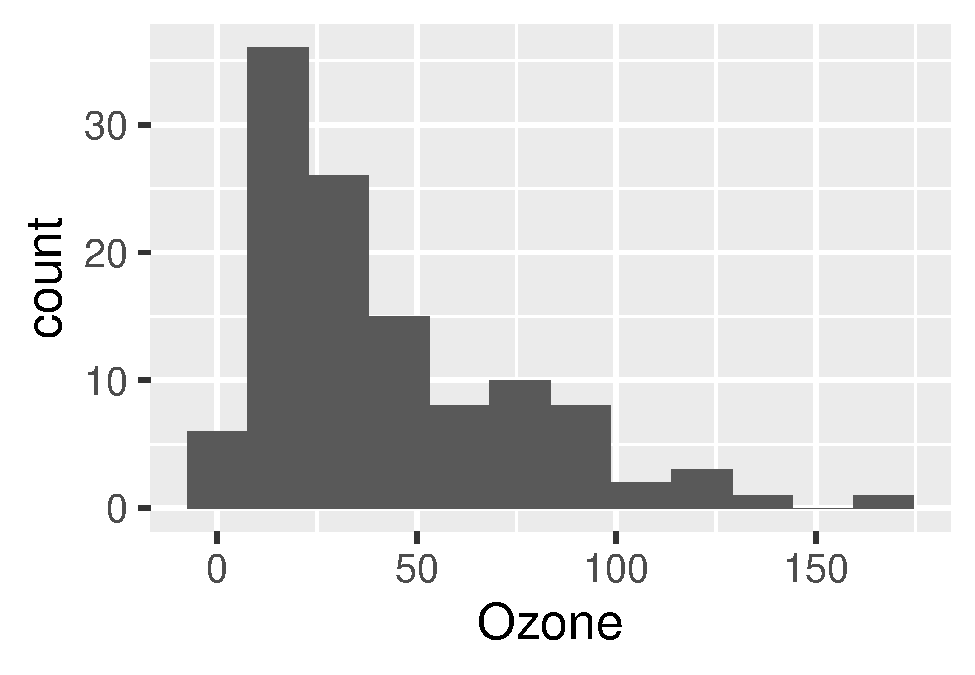
\includegraphics{_main_files/figure-latex/unnamed-chunk-8-1.pdf}

At this point, you can go back and run \texttt{\{targets\}} chunks in interactive mode without interfering with the code or data of the non-interactive pipeline.

\hypertarget{chapter-2}{%
\chapter{Chapter 2}\label{chapter-2}}

Target Markdown is a powerful R Markdown interface for reproducible analysis pipelines, and the chapter at \url{https://books.ropensci.org/targets/markdown.html} walks through it in detail. This R Markdown report the example from the chapter. Try it out in both interactive and non-interactive modes, either by running the code chunks in different ways or setting the \texttt{tar\_interactive} chunk option.

\hypertarget{packages-1}{%
\section{Packages}\label{packages-1}}

The example requires several R packages, and \texttt{targets} must be version 0.5.0.9000 or above.

\begin{Shaded}
\begin{Highlighting}[]
\FunctionTok{install.packages}\NormalTok{(}\FunctionTok{c}\NormalTok{(}\StringTok{"biglm"}\NormalTok{, }\StringTok{"dplyr"}\NormalTok{, }\StringTok{"ggplot2"}\NormalTok{, }\StringTok{"readr"}\NormalTok{, }\StringTok{"targets"}\NormalTok{, }\StringTok{"tidyr"}\NormalTok{))}
\end{Highlighting}
\end{Shaded}

\hypertarget{targets-1}{%
\section{Targets}\label{targets-1}}

Our next targets preprocess the data, make a histogram, and fit a model.

\begin{Shaded}
\begin{Highlighting}[]
\FunctionTok{list}\NormalTok{(}
  \FunctionTok{tar\_target}\NormalTok{(hist2, }\FunctionTok{create\_plot}\NormalTok{(data))}
\NormalTok{)}
\CommentTok{\#\textgreater{} Establish \_targets.R and \_targets\_r/targets/downstream{-}targets2.R.}
\end{Highlighting}
\end{Shaded}

Set the \texttt{tar\_simple} chunk option to \texttt{TRUE} to define a single target with the command in the code chunk. The chunk below only contains \texttt{biglm(Ozone\ \textasciitilde{}\ Wind\ +\ Temp,\ data)} in the source, but because \texttt{tar\_simple} is \texttt{TRUE}, it is shorthand for \texttt{tar\_target(name\ =\ fit,\ command\ =\ biglm(Ozone\ \textasciitilde{}\ Wind\ +\ Temp,\ data))}. All other arguments to \texttt{tar\_target()} are set to their default values (configurable with \texttt{tar\_option\_set()}).

\begin{Shaded}
\begin{Highlighting}[]
\FunctionTok{tar\_target}\NormalTok{(fit2, \{}
  \FunctionTok{biglm}\NormalTok{(Ozone }\SpecialCharTok{\textasciitilde{}}\NormalTok{ Wind }\SpecialCharTok{+}\NormalTok{ Temp, data)}
\NormalTok{\})}
\CommentTok{\#\textgreater{} Define target fit2 from chunk code.}
\CommentTok{\#\textgreater{} Establish \_targets.R and \_targets\_r/targets/fit2.R.}
\end{Highlighting}
\end{Shaded}

\hypertarget{pipeline-1}{%
\section{Pipeline}\label{pipeline-1}}

If you ran all the \texttt{\{targets\}} chunks in non-interactive mode, then your R scripts are set up to run the pipeline.

\begin{Shaded}
\begin{Highlighting}[]
\FunctionTok{tar\_make}\NormalTok{()}
\CommentTok{\#\textgreater{} ✓ skip target raw\_data}
\CommentTok{\#\textgreater{} ✓ skip target data}
\CommentTok{\#\textgreater{} ✓ skip target fit2}
\CommentTok{\#\textgreater{} ✓ skip target fit}
\CommentTok{\#\textgreater{} ✓ skip target hist}
\CommentTok{\#\textgreater{} ✓ skip target hist2}
\CommentTok{\#\textgreater{} ✓ skip pipeline}
\CommentTok{\#\textgreater{} Warning message:}
\CommentTok{\#\textgreater{} package ‘targets’ was built under R version 4.1.2}
\end{Highlighting}
\end{Shaded}

\hypertarget{output-1}{%
\section{Output}\label{output-1}}

You can retrieve results from the \texttt{\_targets/} data store using \texttt{tar\_read()} or \texttt{tar\_load()}.

\begin{Shaded}
\begin{Highlighting}[]
\FunctionTok{library}\NormalTok{(biglm)}
\FunctionTok{tar\_read}\NormalTok{(fit2)}
\CommentTok{\#\textgreater{} Large data regression model: biglm(Ozone \textasciitilde{} Wind + Temp, data)}
\CommentTok{\#\textgreater{} Sample size =  116}
\end{Highlighting}
\end{Shaded}

\begin{Shaded}
\begin{Highlighting}[]
\FunctionTok{tar\_read}\NormalTok{(hist2)}
\end{Highlighting}
\end{Shaded}

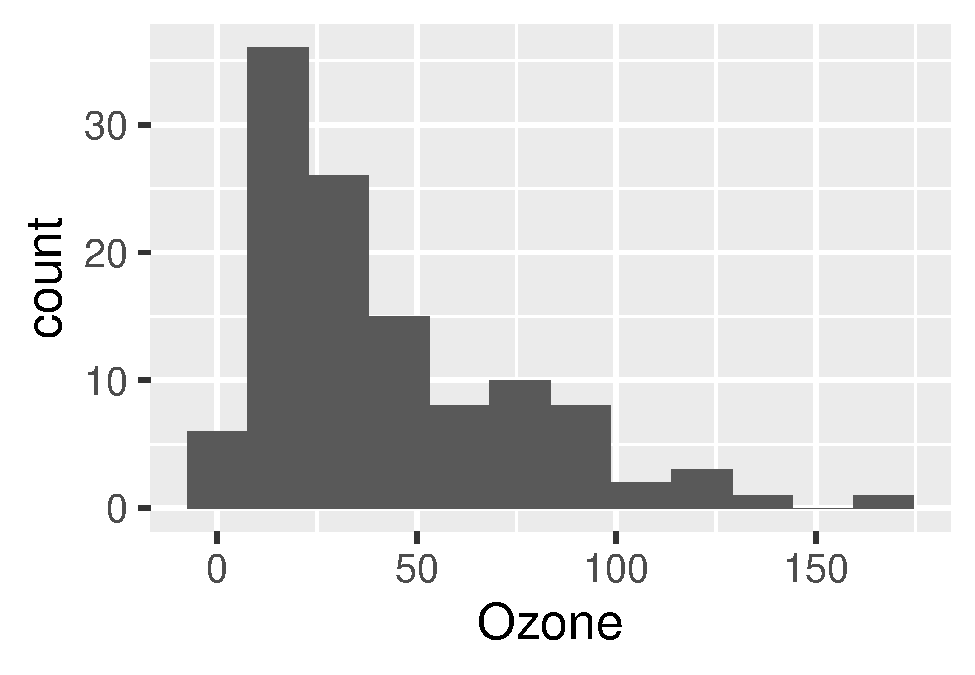
\includegraphics{_main_files/figure-latex/unnamed-chunk-12-1.pdf}

At this point, you can go back and run \texttt{\{targets\}} chunks in interactive mode without interfering with the code or data of the non-interactive pipeline.

  \bibliography{book.bib,packages.bib}

\end{document}
